\documentclass{article}

\usepackage{amsthm}
\newtheorem{proposition}{Proposition}[section]
\theoremstyle{definition}
\newtheorem{definition}{Definition}[section]
\newtheorem{theorem}{Theorem}[section]
\newtheorem{example}{Example}[section]
\theoremstyle{remark}
\newtheorem{remark}{Remark}[section]
\newtheorem{lemma}{Lemma}[section]

\setlength{\parskip}{0.5em}

\usepackage[linesnumbered,ruled,vlined]{algorithm2e}
\usepackage{comment}
\usepackage{pgf}
\usepackage{tikz}
\usetikzlibrary{arrows,automata}
\usepackage[utf8]{inputenc} 		% encodage des caracteres utilise (pour les caracteres accentues) -- non utilise ici.
%\usepackage[latin1]{inputenc} 		% autre encodage
\usepackage[english]{babel}		% pour une mise en forme "anglaise"
\usepackage{amsmath,amssymb,amsthm}	% pour les maths
\usepackage{graphicx}			% pour inclure des graphiques
\usepackage{hyperref}			% si vous souhaitez que les references soient des hyperliens
\usepackage{color}			% pour ajouter des couleurs dans vos textes
\usepackage{todonotes}

\def \N {\mathbb N}	


\title{Implementing the Core Chase for the Description Logic ALC}
\author{Maël Abily}	


\newcommand{\TodoDavid}[1]{\todo[color=green!40]{#1}}
\newcommand{\TodoJF}[1]{\todo{#1}}

\newcommand{\Vars}{\textbf{Vars}}
\newcommand{\Terms}{\textbf{Terms}}
\newcommand{\Preds}{\textbf{Preds}}
\newcommand{\Csts}{\textbf{Csts}}
\newcommand{\Merge}{\textit{Merge}}
\newcommand{\Depth}{\textit{depth}}
\newcommand{\Appl}{\textbf{appl}}
\newcommand{\father}{\textbf{father}}
\newcommand{\Tree}{\textit{Tree}}
\newcommand{\Fut}{\textbf{Fut}}
\newcommand{\su}{\textbf{Succ}}



\begin{document}
\maketitle						% Genere le titre



\section{Introduction}

An important problem in database is the conjunctive query entailment. This problem can be described in a first order logic background: Given a knowledge base $O = (R,F)$ where $F$ is a set of conjunctive formulas (that are formulas constructed only with conjunction and existential quantification) and $R$ is a set of  rules (that are formulas of the form $\forall \vec x.\forall \vec y.( A(\vec x,\vec y) \rightarrow \exists \vec z. B(\vec x,\vec z))$ where $\vec u$ represents a tuple of variables), and given a query $Q$ (that is a conjunctive formula), determine if the knowledge base $O$ entails the query $Q$. We usually use reasoning algorithms to answer this problem. We can notice that in practice, a lot of formulas can be express via conjunctive formulas.

\begin{example}
For the knowledge base $O$ composed of the set of conjunctive formulas $F = \{\textit{Father}(\textit{Michel}) \}$ and the set of rules $R= \{\forall x. \textit{Father}(x) \rightarrow \exists y. \textit{IsTheSonOf}(y,x) \}$, and for the query $Q = \exists y. \textit{IsTheSonOf}(y,Michel)$, the knowledge base $O$ entails $Q$.
\end{example}

By definition, a knowledge base $O$ entails a query $Q$ if every  model of $O$ is a model of $Q$. It is not practical because a knowledge base can have an infinite number of model.

To deal with this problem, we can compute an universal model of the knowledge base $O$. That is a model of $O$ that is entailed by all the models of $O$. If a such model $U$ exists, we just need to show that $U$ entails $Q$ to conclude that $O$ entails $Q$. Hence, to solve query entailment, we just have to compute a finite universal model $U$ for a given input knowledge base and look if $U$ entails $Q$.

To compute these models, we can use algorithms called the chase. We will present in this document the oblivious chase, the restricted chase and then the core chase. The last chase is the best in the sense of it terminates if and only if there exists a finite universal model. 

Nevertheless, it is the slowest so it it is never used for practical applications.

Therefore, we will focus on a restricted type of knowledge base $O=(R,F)$ where the set of conjunctive formulas $F$ is ground (that is there is no variable in the formula) and where the rule contained in $R$ are Horn-$\mathcal{ALC}$ axioms. It is an interesting restriction because we can represent the results of the chase by a tree.

We will create a quicker chase, that we called the merge chase, that would produce the same output than the core chase. It is based on the idea that in a tree, there exists a sibling relation between the nodes (that is two nodes are siblings if they have the same father) and we will see that, in some conditions, a sibling of a node can be merged on this node like in the figure below where $y$ is a sibling of $t'$ and is merged on it.


\begin{center}
\begin{tikzpicture}[scale=0.2]
\tikzstyle{every node}+=[inner sep=0pt]

\draw [white] (17.1,-35.9) circle (3);
\draw (17.1,-35.9) node {$t_0$};
\draw [white] (10.1,-24.1) circle (3);
\draw (10.1,-24.1) node {$t'$};
\draw [white] (24.1,-24.1) circle (3);
\draw (24.1,-24.1) node {$y$};
\draw [white] (24.1,-12.4) circle (3);
\draw (24.1,-12.4) node {$x$};
\draw [white] (10.1,-12.4) circle (3);
\draw (10.1,-12.4) node {$t$};
\draw [white] (30.7,-24.6) circle (3);
\draw [white] (50.4,-24.6) circle (3);
\draw [white] (59.7,-36.8) circle (3);
\draw (59.7,-36.8) node {$t_0$};
\draw [white] (59.7,-25.3) circle (3);
\draw (59.7,-25.3) node {$t'$};
\draw [white] (53.4,-13.2) circle (3);
\draw (53.4,-13.2) node {$t$};
\draw [white] (65.4,-13.2) circle (3);
\draw (65.4,-13.2) node {$x$};
\draw [black] (15.57,-33.32) -- (11.63,-26.68);
\fill [black] (11.63,-26.68) -- (11.61,-27.62) -- (12.47,-27.11);
\draw (14.25,-28.75) node [right] {};
\draw [black] (10.1,-21.1) -- (10.1,-15.4);
\fill [black] (10.1,-15.4) -- (9.6,-16.2) -- (10.6,-16.2);
\draw (10.6,-18.25) node [right] {};
\draw [black] (18.63,-33.32) -- (22.57,-26.68);
\fill [black] (22.57,-26.68) -- (21.73,-27.11) -- (22.59,-27.62);
\draw (21.25,-31.25) node [right] {};
\draw [black] (24.1,-21.1) -- (24.1,-15.4);
\fill [black] (24.1,-15.4) -- (23.6,-16.2) -- (24.6,-16.2);
\draw (24.6,-18.25) node [right] {};
\draw [black] (33.7,-24.6) -- (47.4,-24.6);
\fill [black] (47.4,-24.6) -- (46.6,-24.1) -- (46.6,-25.1);
\draw [black] (59.7,-33.8) -- (59.7,-28.3);
\fill [black] (59.7,-28.3) -- (59.2,-29.1) -- (60.2,-29.1);
\draw (60.2,-31.05) node [right] {};
\draw [black] (58.31,-22.64) -- (54.79,-15.86);
\fill [black] (54.79,-15.86) -- (54.71,-16.8) -- (55.6,-16.34);
\draw (57.24,-18.11) node [right] {};
\draw [black] (60.98,-22.59) -- (64.12,-15.91);
\fill [black] (64.12,-15.91) -- (63.33,-16.42) -- (64.23,-16.85);
\draw (63.26,-20.3) node [right] {};
\end{tikzpicture}
\end{center}

We will then try to extend the merge chase on other type of knowledge bases.

\tableofcontents			

First of all, we will define the usefull notions for this paper and give some well known properties. Then, we will move on our contributions. 

\section{Background}

This section deals with a lot of first order logic notions like interpretations and formulas.

\subsection{Facts}

\subsubsection{Syntax}

We considered a set of variables \Vars\ (often noted $x,y,x_{1},\ldots$), a set of constants \Csts\ (often noted $a,b,c,c_{1},\ldots$), and a set of predicates \Preds\ $(P,Q,R,P_{1},\ldots)$. \Csts, \Vars, and \Preds\ are pairwise disjoint. A \emph{term}  (often noted $t,t_{1},\ldots$) is a variable or a constant. We note \Terms\ the set of terms.  

\begin{definition}
If $t_1,\ldots,t_n$ are terms and $P$ is a predicate of arity $n$, then $P(t_{1},\ldots,t_{n})$ is an \emph{atom}. The atom $P(t_{1},\ldots,t_{n})$ is \emph{ground} if $t_1,\ldots,t_n$ are constants.
\end{definition}

\begin{definition}
A \emph{factbase} $F$ is an existentially closed conjunction of atoms, that is, a formula that does not contain occurrences of free variables and is of the form $\exists x_{1},\ldots,x_{n}.P_{1}(t_{1}^{1},\ldots,t_{k_{1}}^{1})\land \ldots\land P_{m}(t_{1}^{m},\ldots,t_{k_{m}}^{m})$ where $t_i^j$ are terms and $P_i$ are predicates. A factbase is \emph{ground} if each of its atoms is ground.
\end{definition}

In some articles, the factbases are always considered as ground but in this document, we consider factbases that may not be ground. Consequently, a  boolean conjonctive query will be a factbase, so we will only talk about factbases and not introduce the notion of query.

For convenience, we identify factbases as sets of atoms, which allows us to  use  set  notions  such  as  set inclusion. For example, we identify the factbase $$\exists x,x_{1},x_{2},x_{3}. P(x) \land Q(x,a) \land R(x_{1},x_{2},x_{3},b)$$ with the set of facts $$\{P(x),Q(x,a),R(x_{1},x_{2},x_{3},b)\}$$

For a formula $A$, let \emph{$\Vars(A)$}, \emph{$\Csts(A)$}, and \emph{$\Terms(A)$} be the sets of variables, constants, and terms that occur in $A$, respectively.

\begin{definition}
A factbase $F$ \emph{entails} another factbase $F'$ (often noted $F \models F'$) if each interpretation satisfying $F$ satisfies $F'$.
\end{definition}	

\begin{definition}
A factbase $F$ is equivalent to another factbase $F'$ if $F \models F'$ and $F' \models F$.
\end{definition}

\subsubsection{Homomorphism}

\begin{definition}[Substitution]
A \emph{substitution} $\sigma:X \to \Terms$ is a function where X is a set of variables. For example $\{x \mapsto z, y \mapsto a \}$ is a substitution from $\{x,y\}$ to \Terms. By extension: 
\begin{itemize}
\item if $c \in \Csts$, then $\sigma(c) = c$;
\item if $x \in \Vars \setminus X$, $\sigma(x) = x$;
\item if $f = P(t_1,\ldots,t_n)$ is an atom, then $\sigma(f) = P(\sigma(t_1),\ldots,\sigma(t_n))$; and
\item if $F = \{f_1,\ldots,f_n\}$ is a factbase, then $\sigma(F) = \{\sigma(f_1),\ldots,\sigma(f_n)\}$.
\end{itemize}
\end{definition}

\begin{definition}
For two factbases $F$ and $F'$, a \emph{homomorphism} from $F$ to $F'$ is a substitution $\sigma:\Vars(F) \to \Terms$ where $\sigma(F) \subseteq F'$. Sometimes, we will say that we \emph{map} a variable $x$ to a term $t$ if $\sigma(x)=t$.
\end{definition}

\begin{definition}
For two factbases $F$ and $F'$, an \emph{isomorphism} $h$ from $F$ to $F'$ is a bijective homomorphism where its inverse is a homomorphism from $F'$ to $F$. 
\end{definition}

For the remainder of this paper, we identify sets of facts that are unique up to isomorphism.

%\begin{remark}
%A bijective homomorphism is not necessarily an isomorphism. For example, 
%\begin{align*}
%\sigma:\{R(x)\} &\to \{R(a)\}\\
%x &\mapsto a
%\end{align*}
%is a bijective homomorphism but not an isomorphism.
%\end{remark}



\begin{theorem}[Homomorphism Theorem] \label{hom_thm}
A factbase $F$ \emph{entails} another factbase $Q$ if and only if there exists a homomorphism from $Q$ to $F$.
\end{theorem}

The previous theorem has been proved in (\cite{base},theorem 6.2.3).

\begin{example}
The factbase $F = \{P(b,a),A(x)\}$ entails the factbase $Q = \{P(x,a),P(y,z)\}$ due to the homomorphism $\{x \mapsto b, y \mapsto b, z \mapsto a \}$.
\end{example}




%\begin{proof} The size of the problem is $\textit{card}(\Terms(F))+\textit{card}(\Terms(Q))$.
%\begin{itemize}
%\item We choose, as certificate, a homomorphism $\sigma$ from $Q$ to $F$. Firstly, the size of the certificate is $card(var(Q))+ card(terms(F))$ which is polynomial in the size of the problem. Secondly, we can check that the certificate $\sigma$ is a homomorphism in a time which is polynomial in the size of the problem. Therefore, the problem is in NP.  
%\item We make a reduction from 3-COLOR which is known to be NP-complete. Let $G= (V,E)$ be a graph. Let $P$ be a binary predicate. We pose $Q_G = \{P(x,y)/(x,y) \in E\}$ and $K_3 = \{P(c_1,c_2),P(c_1,c_3), P(c_2,c_1),P(c_3,c_1),\\P(c_2,c_3),P(c_3,c_2)\}$. We have to show that $K_3 \models Q_G \Leftrightarrow$ $G$ is 3-colorable. \\
%$\boxed{\Rightarrow}$ Suppose that $K_3 \models Q_G$. There exists a substitution $\sigma:Q_G \to K_3$. We pose: 
%\begin{align*}
%c:V &\to \{c_1,c_2,c_3\}\\
%x &\mapsto \sigma(x)
%\end{align*}
%if $(x,y) \in E$, $P(x,y) \in Q_G$ and so $P(\sigma(x),\sigma(y)) \in K_3$, so $c(x) \neq c(y)$. Therefore, $c$ is a 3-coloration of $G$. \\
%$\boxed{\Leftarrow}$ Conversely, suppose that $G$ is 3-colorable. Let $c:V \to \{c_1,c_2,c_3\}$ be a coloration of $G$. $c$ is a substitution from $Q_G$ to $K_3$. We have to show that $c(Q_G) \subset K_3$. Let $P(x,y)$ be in $Q_G$. We have $(x,y) \in E$, so $c(x) \neq c(y)$. So $P(c(x),c(y)) \in K_3$. Therefore, $c$ is a homomorphism from $Q_G$ to $K_3$ and so $K_3 \models Q_G$.
%\end{itemize}
%\end{proof}




\subsubsection{Core}

For a factbase $F$, let $id_{|F}$ be the substitution mapping each variable in $\Vars(F)$ to itself. And for a subsitution $\sigma$ defined on a factbase $F'$ containing $F$, let $\sigma_{|F}$ be the subsitution $\sigma$ defined only on $\Vars(F)$. In practice, it is better to work on smaller factbases. It leads us to the notions of retracts and cores:

\begin{definition}
A factbase $F'$ is a \emph{retract} of another factbase $F$ if $F' \subseteq F$ and $F' \models F$. A \emph{retractation} from $F$ to $F'$ is a homomorphism $\sigma$ from $F$ to $F'$ such that $\sigma_{|F'}=id_{|F'}$. $F'$ is a \emph{strict retract} of $F$ if $F'$ is a retract of $F$ and $F' \neq F$.
\end{definition}


\begin{proposition} \label{retract}
The factbase $F'$ is a retract of the factbase $F$ if and only if $F' \subseteq F$  and there exists a retractation from $F$ to $F'$.
\end{proposition}

\begin{definition}
If a factbase $F$ does not contain a strict retract, then we say that $F$ is a \emph{core}. A \emph{core} of a factbase $F$ (noted \emph{$\textit{core}(F)$}) is a subset of $F$ that is a core.
\end{definition}

\begin{proposition}
The cores of a finite factbase F are unique up to isomorphism.
\end{proposition}

Hence, we speak of ``the'' core of a factbase.

\begin{example}
$F_1 = \{B(x,y),R(y,z)\}$ is the core of $$F = \{B(x,y),R(y,z),B(x,w),R(w,z)\}$$ because:
\begin{itemize}
\item $F_1 \subseteq F$;
\item $\{x \mapsto x, y \mapsto y, z \mapsto z, w \mapsto y\}$ is a homomorphism from $F$ to $F_1$, so $F_1$ is a retract of $F$;
\item all strict subsets of $F_1$ are not retracts of $F_1$.
\end{itemize}
Note that $F_2 = \{B(x,w),R(w,z)\}$ is also the core of $F$ and is indeed isomorphic to $F_1$ due to the homomorphism $\{x \mapsto x, y \mapsto w, z \mapsto z\}$ .
\end{example}

%\begin{proposition}
%A factbase $F$ is a core $\Leftrightarrow$ every homomorphism $\sigma$ from $F$ to $F$ is a bijection.
%\end{proposition} 

%\begin{proof}
%We show it by double-implication. \\
%$\boxed{\Leftarrow}$ By contraposition, suppose that the factbase $F$ is not a core: there exists a strict substet $F'$ of $F$ such that $F'$ is a retract of $F$. There exists a homomorphism $\sigma:F \to F$ such that $\sigma(F) = F'$. As $F' \subsetneq F$, $\sigma$ is not surjective, so it is not a bijection. \\
%$\boxed{\Rightarrow}$ Conversely, by contraposition, suppose that there exists a homomorphism $\sigma_1$ that is not bijective. As $F$ is finite, $\sigma_1$ is not surjective. We pose $F' = \sigma_1(F)\subsetneq F$ and we pose $\sigma_2:F \to F$ such that for $x \in F'$, $\sigma_2(x) = x$ and for $x \notin F'$, $\sigma_2(x) = \sigma_1(x)$. We have ${\sigma_2}_{|F'} = id_{|F'}$ and $\sigma_2(F) = F'$. So $\sigma_2$ is a retractation from $F$ to $F'$ and so $F'$ is a strict retract of $F$. Consequently $F$ is not a core.
%\end{proof}



\subsection{Existential Rules}

\subsubsection{Syntax}

\begin{definition}
Let $\vec x$, $\vec y$, and $\vec z$ be some tuples of variables that are pairwise disjoint. An \emph{(existential) rule} $\alpha$ is a first-order formula	of the form $$\forall \vec x.\forall \vec y.( A(\vec x,\vec y) \rightarrow \exists \vec z. B(\vec x,\vec z))$$ where $A$ and $B$ are conjunctions of atoms. We define \emph{$\textit{body}(\alpha)$} = $A$ and \emph{$\textit{head}(\alpha)$} = $B$.
\end{definition}
We omit the universal quantifiers when representing existential rules.
\begin{definition}

A \emph{knowledge base} $O$ is a pair $(R,F)$ where $R$ is a set of existential rules and $F$ is a  ground factbase.
\end{definition}


\subsubsection{Semantics}

\begin{definition}[Entailment]
A factbase $F$ \emph{entails} a rule $\alpha$ if each interpretation satisfying $F$ satisfies $\alpha$. We will note $F \models R$ if $F$ entails each rule of the rule set $R$.
\end{definition}

\begin{theorem}
A factbase $F$ \emph{entails} a rule $\alpha = A(\vec x,\vec y) \rightarrow \exists \vec z. B(\vec x,\vec z)$ if and only if for every homomorphism $\sigma$ from $A$ to $F$, there exists an extension of $\sigma$ that is a homomorphism from $B$ to $F$.
\end{theorem}



\begin{definition}[Model]
A factbase $M$ is a \emph{model} for a knowledge base $O = (R,F)$ if $M \models F$ and $M \models R$.
\end{definition}




\begin{example} We pose $O = (\{\alpha\},F)$ where $\alpha = A(x) \rightarrow \exists z.R(x,z) \wedge A(z)$ and $F = \{A(b)\}$. An universal model of $O$ is $$U = \{A(b),R(b,x_0)\}\cup \{A(x_i)\mid i \in \N\}\cup \{R(x_i,x_{i+1}) \mid i \in \N\}$$ The knowledge base $O$ does not admit finite universal models.
\end{example}

\begin{definition}[Entailment]
A knowledge base $O$ \emph{entails} a factbase B (often noted $O \models B$) if for each model $M$ of $O$, $M \models B$.
\end{definition}

\begin{definition}[Universal model]
A factbase $U$ is an \emph{universal model} for a knowledge base $O = (R,F)$ if for
every model $M$ of $O$, $M \models U$.
\end{definition}


We are interested by universal models because  they can be used to solve fact entailment:

\begin{proposition}
A knowledge base $O$ entails a factbase $B$ if there exists a universal model $U$ for $O$ such that $U \models B$.
\end{proposition}

An important problem that this document has to deal with is: Given a knowledge base $O=(R,F)$ and a factbase $Q$,  does $O \models Q$? It  is  well-known  that  this  problem  is  undecidable (\cite{NP2}, theorem 4). 



\subsection{The Chase}

The process of applying rules on a factbase in order to infer more knowledge is called forward chaining.   Forward  chaining  in  existential  rules  is  usually achieved  via  a  family  of  algorithms  called the  chase. It can be seen as a two-steps process. It first repeatedly applies rules to the set of facts (and eventually computes sometimes the core to supress redundant facts). Then it looks for an answer to the query in this saturated set of facts. This saturated set of facts is a universal model of the knowledge base. The chase is sound and complete; so it must be non-terminating since the problem of entailment is undecidable. To determine how we apply a rule to a set of fact, we introduce the notion of trigger:

\begin{definition}[Trigger]
Let $T$ be a rule set, $\alpha$ be a rule, $\sigma$ be a substitution, and $F$ be a factbase. The tuple $t = (\alpha,\sigma)$ is an \emph{oblivious trigger} for $F$ if: 
\begin{itemize}
\item the domain of $\sigma$ is the set of all variables occurring in $Body(\alpha)$.
\item $\sigma$ is a homomorphism from $Body(\alpha))$ to $F$.
\end{itemize}
In this case, we say that $t$ is \emph{applicable} on $F$.

The tuple $t = (\alpha,\sigma)$ is a \emph{restricted trigger} for $F$ if $t$ is an oblivious trigger for $F$ and if for all $\hat \sigma$ that extend $\sigma$ over $\Vars(\textit{Head}(\alpha))$, $\hat \sigma(Head(\alpha)) \nsubseteq F$.
\end{definition} 



Notice that a restricted trigger is also an oblivious trigger. We will therefore use the term trigger to talk about the oblivous and the restricted trigger.

The chase will considere triggers to infer new knowledge from an initial factbase. We explain now how it would apply a trigger, giving rise to the notion of application. 

\begin{definition}[application]
For a trigger $t = (\alpha,\sigma)$ for the factbase $F$ where $\alpha$ is of the form $A(\vec x,\vec y) \rightarrow \exists \vec z. B(\vec x,\vec z)$, we pose \emph{$\sigma^s$} the substitution that extends $\sigma$ over $\Vars(\textit{Head}(\alpha))$ such that for $z \in \vec z$, $\sigma^s(z) = f^z_\alpha(\sigma(\vec x))$ where $f^z_\alpha(\sigma(\vec x))$ is a fresh variable unique with respect to the trigger $t$ and the variable $z$.
The factbase $\Appl(F,t)=F \cup \sigma^s(\textit{Head}(\alpha))$ is called an \emph{application} on the factbase $F$ through the trigger $t = (\alpha,\sigma)$. 

We say that the trigger $t$ \emph{has been applied} on $F$ if $\Appl(F,t) = F$.
\end{definition}



\begin{example}. If $\alpha = A(x,y) \rightarrow \exists z.B(x,z)$, $F = \{A(b,c)\}$, and $\sigma = \{x \mapsto b, y \mapsto c \}$ then $(\alpha,\sigma)$ is a restricted trigger for $F$. We have $$\Appl(F,(\alpha,\sigma)) = \{A(b,c),B(b,f_{\alpha}^z(b,c)\}$$
\end{example}

\begin{definition}[Derivation]
An \emph{oblivious derivation} (respectively a \emph{restricted derivation}) for a knowledge base $O= (F,R)$ is a (possibly infinite) sequence $D=F_0,t_1,F_1,t_2,F_2,\ldots$ where 
\begin{itemize}
\item $F_0,F_1,\ldots$ are factbases such that $F_i \subsetneq F_{i+1}$.
\item $t_1,t_2,\ldots$ are oblivious triggers (resp. restricted triggers).
\item $F_0 = F$.
\item For all $i > 0$, $F_{i}= \Appl(F_{i-1},t_i)$.
\end{itemize}
\end{definition}


\begin{definition}[Fairness]
The oblivious (resp. restricted) derivation $D=F_0,t_1,F_1,t_2,F_2,\ldots$ is \emph{fair} if for every $i$ and every oblivious (resp. restricted) trigger $t$ for $F_i$, there exists $k \geq i$ such that $\Appl(F_{k},t_k) = F_k$ (resp. $t$ is not anymore a restricted trigger for $F_k$).
\end{definition}

A fair derivation garantees that we consider every possible application. An easy way to have a fair derivation is to do a breadth-first search (BFS) on the terms, that is, always apply the oldest triggers before applying other triggers.

We will now define the oblivious and restricted chase, It is defined in \cite{obl_res}.


\begin{definition}
An \emph{oblivious chase} (resp. a restricted chase) for a knowledge base $O= (F,R)$ is a fair oblivious (resp. restricted) derivation $D=F_0,t_1,F_1,t_2,F_2,\ldots$ 
\end{definition}

For every oblivious chase $D = F_0,t_1,F_1,t_2,F_2,\ldots$ for $O$, we have $F_0 \subseteq F_1 \subseteq F_2 \subseteq \ldots$. The result of an oblivious chase does not depend on the derivation $D$ so we can pose \emph{$\textit{Obl(O)}$} = $\cup_{i \in \N}F_i$. We say that the oblivious chase \emph{terminates} if $\textit{Obl(O)}$ is finite.

It is well known that:

\begin{theorem}
For a knowledge base $O$, $\textit{Obl}(O)$ is an universal model of $O$.
\end{theorem}

Consequently, the oblivious chase can be used to solve query entailment.

It is more difficult to define the result of the restricted chase because the result depends on the order of the application of the rules. We define $$\textit{Res(O)}=\{\cup_{i \in \N}F_i \mid D = F_0,t_1,F_1,t_2,F_2,\ldots \text{is a retricted chase for } O\}$$

We say that the restricted chase \emph{terminates} if there exists an element in $\textit{Res(O)}$ that is finite.

It is well known that:

\begin{theorem}
For a knowledge base $O$ and for every $U \in \textit{Res}(O)$, $U$ is an universal model of $O$.
\end{theorem}


The oblivious chase  can do a lot of applications that are useless: 
\begin{example}
Suppose that we have the knowledge base $O=(\{\alpha\},F)$ where $\alpha = A(x,y) \rightarrow \exists z.A(y,z) \wedge A(z,y)$ and $F =  \{A(a,b)\}$. An oblivious chase derivation is $F_0,t_1,F_1,t_2,F_2,...$ where
\begin{itemize}
\item $F_0 = F$, 
\item $t_1=(\alpha,\{x \mapsto a, y \mapsto b\})$, 
\item $F_1=\{A(a,b),A(b,z_1),A(z_1,b)\}$ where $z_1 =f_\alpha^z(a,b)$,
\item $t_2=(\alpha,\{x \mapsto b, y \mapsto z_1\})$, 
\item $F_2=F_1 \cup \{ A(z_1,z_2), A(z_2,z_1)\}$ where $z_2= f_\alpha^z(b,z_1)$, 
\item \ldots\ 
\end{itemize} 
It will never terminate because each new atom brings new rule applications. So the oblivious chase does not terminate on $O$ whereas the restricted chase terminates. A restricted chase derivation is $F_0,t_1,F_1$ where $F_0 = F$, $t_1=(\alpha,\{x \mapsto a, y \mapsto b\})$, and $F_1=\{A(a,b)$,$A(b,z_{t_1})$, $A(z_{t_1},b)\}$. This derivation is fair because there is not anymore any restricted trigger for $F_1$. We have $F_1 \in \textit{Res(O)}$.
\end{example}




\begin{theorem}
A knowledge base $O$ entails a factbase $B$ if and only if $\textit{Obl}(O) \models B$ and $O$ entails $B$ if and only if for every $U \in \textit{Res}(O)$, $U \models B$.
\end{theorem}




\subsubsection{The core chase}

It has been firstly defined in \cite{core_chase}.

\begin{definition}[Core derivation]
A \emph{core derivation} for a knowledge base $O = (R,F)$ is a (possibly infinite) sequence $D = F_0, F_1, F_2, \ldots$ where $F_0 = F$, and for $i >0$, either $F_{i}= \Appl(F_{i-1},t_i)$ is obtained by an application with $t_i$ an oblivious trigger, or $F_i$ is the core of $F_{i-1}$. 
\end{definition} 

\begin{definition}[Fairness]
A core derivation $D=F_0,F_1,F_2,\ldots$ is \emph{fair} if:
\begin{itemize}
\item For every $i$, for every oblivious trigger $t$ for $F_i$, there exists $k \geq i$ such that $\Appl(F_{k},t) = F_k$.
\item For every $i$, there exists $k \geq i$ such that $F_k$ is a core.

\end{itemize}
\end{definition}

\begin{definition}
A \emph{core chase} for a knowledge base $O= (R,F)$ is a fair core derivation $D=F_0,F_1,F_2,\ldots$ The core chase \emph{terminates} on $O$ if it is a finite core derivation.
\end{definition}

The article \cite{core_chase} has proven that the result of the core chase on a knowledge base is unique up to isomorphism. Therefore, we can define the result of the core chase:

\begin{definition}
If the core chase terminates on $O$ due to the finite core derivation $D=F_0,F_1,F_2,\ldots,F_i$, then we pose \emph{$\textit{C}(O)$} = $F_i$. Otherwise, if the core chase does not terminate,$\textit{C}(O)$ is undefined.
\end{definition}

The following theorem has been proven in (\cite{core_chase}, theorem 7)

\begin{theorem}
The knowledge base $O = (R,F)$ admits a finite universal model if and only if the core chase algorithm terminates on $O$.
\end{theorem}


There exists knowledge bases where the restricted chase does not terminate whereas the core chase terminates. \begin{example}
Suppose that we have the knowledge base $O=(\{\alpha\},F)$ where $\alpha = A(x,y) \rightarrow \exists z.(A(x,x) \wedge A(y,z))$ and $F =  \{A(a,b)\}$. A restricted chase derivation is $F_0,t_1,F_1,t_2,F_2,...$ where 
\begin{itemize}
\item $F_0 = F$,
\item $t_1=(\alpha,\{x \mapsto a, y \mapsto b\})$, 
\item $F_1= F_0 \cup \{A(a,a),A(b,z_1)\}$ where $z_1 = f_\alpha^z(a,b)$,
\item $t_2 = (\alpha,\{x \mapsto b, y \mapsto z_1\})$, 
\item $F_2 = F_1 \cup \{A(b,b),A(z_1,z_2)\}$ where $z_2 = f_\alpha^z(b,z_1)$, 
\item $t_3 = (\alpha,\{x \mapsto z_1, y \mapsto z_2\})$, 
\item $F_3 =  F_2 \cup \{A(z_1,z_1),A(z_2,z_3)\}$ where $z_3 = f_\alpha^z(z_1,z_2)$,
\item \ldots\
\end{itemize}
It will never terminate because each new atom brings new restricted triggers. 

The core chase terminates on $O$: a core chase derivation is $F_0,F_1,F_2,F_3,F_4,F_5$ where 
\begin{itemize}
\item $F_0=F$, 
\item $t_1=(\alpha,\{x \mapsto a, y \mapsto b\})$, 
\item $F_1=\Appl(F_0,t_1) =F_0 \cup \{A(a,a),A(b,z_1)\}$ where $z_1 = f_\alpha^z(a,b)$, 
\item $t_2 = (\alpha,\{x \mapsto b, y \mapsto z_1\})$,
\item $F_2 =\Appl(F_1,t_2) =F_1 \cup \{A(b,b),A(z_1,z_2)\}$ where $z_2 = f_\alpha^z(b,z_1)$,
\item $t_3 = \{x \mapsto a, y \mapsto a\}$, $F_3=\Appl(F_2,t_3)$, $t_4 = \{x \mapsto b, y \mapsto b\}$, and $F_4=\Appl(F_3,t_4) = F_2 \cup \{A(a,f_\alpha^z(a,a)),A(b,f_\alpha^z(b,b))\}$
\item $F_5 = \textit{Core}(F_4)= \{A(a,a),A(a,b),A(b,b)\}$.
\end{itemize} 
There is not anymore any oblivious trigger for $F_5$ so the derivation is fair. Consequently the core chase terminates on $O$.

\end{example}

\begin{definition}
For a knowledge base $O$ and an operation that transforms a factbase F in another factbase $f(F)$, we say that this operation \emph{preserves the universality} if for each model $M$ of $O$, $M \models F$ implies $M \models f(F)$. 
\end{definition}

\begin{proposition} \label{universality application}
The application of a rule and computing a core are operations that preserve the universality.
\end{proposition}

\begin{proposition}
For a knowledge base $O$, the result of a chase for $O$ is a universal model if the result is a model of $O$ and if the operations used on the factbases preserve the universality.
\end{proposition}

\section{The Merge Chase}

The core chase always terminates when there exists a finite universal model but this core chase is very expensive in time because computing the core of a factbase is hard. Therefore we are presenting a more efficient way to solve this problem in the particular case of Horn-$\mathcal{ALC}$.

\begin{definition}
For a factbase $F$ and a term $t$, we note \emph{$\Preds^1_F(t)$} the set of unary predicates $P$ such that $P(t)\in F$. For two terms $t$ and $t'$, we note \emph{$\Preds^2_F(t,t')$} the set of binary predicates $P$ such that $P(t,t')\in F$.
\end{definition}

In this section, we only consider factbases with predicates of arity one or two. Hence, we will represent a factbase $F$ by a labelled graph $G = (V,E)$ where $V = \{t \mid t \in \Terms \}$ and $E = \{(t_1,t_2) \mid t_1,t_2 \in \Terms \wedge \Preds_F(t_1,t_2) \neq \emptyset\}$. We label the vertex $v \in V$ by exactly the predicates in $\Preds_F^1(v)$ and we label the edge between the terms $t_1$ and $t_2$ by exactly the predicates in $\Preds^2_F(t_1,t_2)$. For example with $F = \{A(a), B(a),R(a,b),T(a,b),C(b),R(b,z)\}$: \\

\begin{tikzpicture}[->,>=stealth',shorten >=1pt,auto,node distance=2.8cm, semithick]
  \tikzstyle{every state}=[fill=white,draw=none,text=black]

  \node[state]         (A)                    {$a:A,B$};
  \node[state]         (B) [above right of=A] {$b:C$};
  \node[state]         (C) [right of=A] {$z$};

  \path (A) edge              node {R,T} (B)
        (B) edge              node {R} (C);
\end{tikzpicture}


\subsection{Horn-$\mathcal{ALCH}$ }

Horn-$\mathcal{ALCH}$ has been introduced in \cite{Horn-ALC}

\begin{definition}[Horn-$\mathcal{ALCH}$ axioms]
A \emph{Horn-$\mathcal{ALCH}$ axiom} is an existential rule of the form:\todo{of one of the following forms:}
\begin{align}
A_1(x) \wedge A_2(x) &\rightarrow B(x) \\
A(x) \wedge R(x,y) &\rightarrow B(y) \\
A(x) &\rightarrow \exists y.R(x,y) \wedge B(y) \\
R(x,y) \wedge B(y) &\rightarrow A(x) \\
R_1(x,y) \wedge R_2(x,y) &\rightarrow S(x,y)
\end{align}

\end{definition}


We fix $O=(R,G)$ a knowledge base for this section where $R$ is a Horn-$\mathcal{ALCH}$ rule set.

We can notice that all the variables are introduced by a Horn-$\mathcal{ALCH}$\todo{Create a macro for Horn-ALC.} axiom of the form $(3)$.\todo{Note that $(3)$ is the only rule that features existentially quantified variables.}\todo{Use the commands ``href'' and ``label'' to reference items within the align environment.}

We will now introduce some notions in order to introduce the new chase and prove that it does what we want.\todo{A bit informal; be more precise; describe ``what is what we want''.}

\begin{definition}
Let $D = F_0,F_1,\ldots,F_k$ be a chase derivation of the knowledge base $O$. For a term $t$ and a variable $x$ appearing in $F_k$, we say that $t \prec x$ if there exists a rule $\alpha$ and a variable $y$ such that $x= f_\alpha^y(t)$.\todo{Alternatively, you may simply say ``if $x$ is of the form $f(t)$''.}
We write $\prec^+$ to denote the transitive closure of $\prec$. We note \emph{$\su(t)$}$= \{y \in \Vars \mid t = y \vee t \prec^+ y\}$.\todo{I would use ``Desc'' (for descendants) instead of ``Succ''. Note that, usually, we say successors to refer to the immediate descendants.}
\end{definition}

\begin{proposition} 
Let $F$ be a factbase that occurs in a chase derivation of the knowledge base $O$. For a term $t$ and a variable $x$, if there exists a rule $\alpha$ and a variable $y$ such that $x= f_\alpha^y(t)$, then $\alpha$ is of the form $(3)$.\todo{Use the commands ``href'' and ``label'' to reference items within the align environment. }
\end{proposition}\todo{This statement can be generalised: Consider a term $t$ that occurs in a chase derivation of some Horn-$\mathcal{ALCH}$ knowledge base. Then, $t$ is a constant or $t$ is of the form $f^y_\alpha(u)$ where $u$ is a term, $\alpha$ is a rule of the form $(3)$, and $y$ is the (only) existentially quantified variable occurring in $\alpha$.}



\begin{proposition} \label{only one predecessor}
Let $F$ be a factbase that occurs in a chase derivation of the knowledge base $O$. For every variable $x$, there exists exactly one predecessor for $\prec$.
\end{proposition}




\begin{proposition} \label{partial_order}
Let $D = F_0,F_1,\ldots,F_k$ be a chase derivation of the knowledge base $O$. $\prec^+$ is a strict partial order over the set of terms of $F_k$.
\end{proposition}

\begin{proof}
Suppose for a contradiction that there exists a term $t$ such that $t \prec^+ t$. There exists then $n \in \N \setminus \{0\}$ and terms $t_0,\ldots,t_n$ such that $t=t_0 \prec t_1 \prec \cdots \prec t_n = t$. By Proposition \ref{prec equivalence}, there exists rules $\alpha_1,\ldots, \alpha_n$ and variables $v_1,\ldots,v_n$ such that $t_n = f_{\alpha_n}^{v_n}(f_{\alpha_{n-1}}^{v_{n-1}}(\cdots f_{\alpha_1}^{v_1}(t_0)\cdots))$. It is a contradiction since $t_0 = t$ and $t_n=t$.

Therefore $\prec^+$ is irreflexive. By construction, $\prec^+$ is transitive; So $\prec^+$ is a strict partial order

\end{proof}

We have shown in the proof that the graph induced by $\prec$ does not contain any cycle. Therefore, with the last proposition and Proposition \ref{only one predecessor}: 

\begin{proposition}
Let $F$ be a factbase that occurs in a chase derivation of the knowledge base $O$. The graph induced by $\prec$ is a forest of trees.
\end{proposition}

We can now define the notion of tree of a term $t$ that is all the facts containing only variables in $\su(t)$:

\begin{definition}[Tree]
Let $F$ be a factbase that occurs in a chase derivation of the knowledge base $O$. For a term $t$, we pose\todo{For a term $t$ occurring in a chase derivation of the Horn-$ALC$ knowledge base $O$, we pose:} 
\begin{align*}
\Tree_{F}(t) = &\{A(t') \mid A(t') \in F \wedge t' \in \su(t)\} \\
 \cup &\{R(t',x) \mid R(t',x) \in F \wedge t',x \in \su(t)\}
\end{align*}
\begin{align*}
	\Tree_{F}(t) = \{&A(u) \mid A(u) \in F \wedge u \in \su(t)\}~\cup \\
	\{&R(u,x) \mid R(u,x) \in F \wedge u,x \in \su(t)\}
\end{align*}
\end{definition}


%We can then associate the depth of a variable:
%
%\begin{definition}
%Let $F$ be a factbase that occurs in a core chase derivation of the knowledge base $O$. We define the \emph{depth} of a term $t$ by induction:
%\begin{itemize}
%\item 
%\end{itemize}
%\end{definition}

We now define the notion of mergeable variable in order to consider a new operation.\todo{which will later be used to define an operation to efficiently compute cores.}

\begin{definition}[Mergeable variable]
Let $F$ be a factbase that occurs in a chase derivation of the knowledge base $O$. For two terms $t_1$ and $t_2$ such that $t_1 \neq t_2$, $t_1$ is \emph{mergeable} on $t_2$ in $F$ if:
\begin{itemize}
\item $t_1$ is a variable,
\item $\Preds_{F}^1(t_1) \subseteq \Preds_{F}^1(t_2)$,\todo{add ``and''}
\item there exists a term $t$ such that
	\begin{itemize}
	\item $\Preds^2_{F}(t,t_1) \neq \emptyset$, and
	\item $\Preds_{F}^2(t,t_1) \subseteq \Preds_{F}^2(t,t_2)$.
	\end{itemize}\todo{I would remove this last itemize.}
\end{itemize}
In this case, we say that $t_1$ is a \emph{mergeable variable}.
\end{definition}

We imposed that $t_1$ is mergeable on $t_2$ only if $t_1$ is a variable because, we will latter map $t_1$ on $t_2$ and it is not possible to map a constant to another term.\todo{Unclear intuition.}

%Notice that the definition of siblings can be shorted because, due to the form of the Horn-$\mathcal{ALCH}$ axioms, for a term $t$, there exists a unique term $t'$ and a unique binary relation $R$ such that $R(t',t)\in F$. So we can replace the last condition in the definition about the existence of $t$ by: there exists a term $t$ and a predicate $R$ such that $R(t,t_1) \in F$ and $R(t,t_2) \in F$. We write this more complex definition because it works in more general cases.

When $x$ is mergeable on $t$ in $F$, we want to say that all the triggers applied on $x$ and on the $\prec$-successor of $x$ can be or have already been applied on $t$ and on the $\prec$-successor of $t$. Therefore, all the facts containing $x$ and the $\prec$-successor of $x$ are or will be redundant. But we do not want to supress all these facts because we know that if they are not yet in the tree of $t$, they would be computed so we would like to "recycle"\todo{This is how you write something in quotes in Latex: ``recycle''.} these facts. That is this intuition that leads us to define atomic merging:


\begin{definition}[atomic merging]
If a variable $x$ is mergeable on a term $t$ in a factbase $F$, then we note $h_{x/t}$ the substitution defined on $\Vars(F)$ such that for every variable $y$ in $\su(x)$, $h_{x/t}(y)$ is the variable $y$ where the occurence of $x$ is replaced by $t$, and for every variable $y$ not in $\su(x)$, $h(y) = y$. 

The \emph{atomic merging} of $x$ on $t$ in $F$ produces $h_{x/t}(F)$ 
\end{definition}

For example, in the figure below, $f_\alpha^y(a)$ is mergeable on $b$ in the left factbase. The atomic merging of $f_\alpha^y(a)$ on $b$ in this factbase gives the right factbase.

\begin{center}
\begin{tikzpicture}[scale=0.2]
\tikzstyle{every node}+=[inner sep=0pt]
\draw [white] (11.7,-48.7) circle (3);
\draw (11.7,-48.7) node {$a:\mbox{ }A$};
\draw [white] (3.8,-39.5) circle (3);
\draw (3.8,-39.5) node {$b:\mbox{ }A$};
\draw [white] (19,-39.5) circle (3);
\draw (19,-39.5) node {$f_\alpha^y(a):\mbox{ }A$};
\draw [white] (50.9,-48.7) circle (3);
\draw (50.9,-48.7) node {$a:\mbox{ }A$};
\draw [white] (50.9,-39.5) circle (3);
\draw (50.9,-39.5) node {$b:\mbox{ }A$};
\draw [white] (30.2,-39.5) circle (3);
\draw [white] (42.6,-39.5) circle (3);
\draw [white] (19,-30.4) circle (3);
\draw (19,-30.4) node {$f_\alpha^y(f_\alpha^y(a)):\mbox{ }A$};
\draw [white] (50.9,-30.4) circle (3);
\draw (50.9,-30.4) node {$f_\alpha^y(b):\mbox{ }A$};
\draw [white] (3.8,-30.4) circle (3);
\draw (3.8,-30.4) node {$f_\alpha^y(b):\mbox{ }A$};
\draw [white] (19,-21.7) circle (3);
\draw (19,-21.7) node {$f_\alpha^y(f_\alpha^y(f_\alpha^y(a))):\mbox{ }A$};
\draw [white] (50.9,-21.7) circle (3);
\draw (50.9,-21.7) node {$f_\alpha^y(f_\alpha^y(b)):\mbox{ }A$};
\draw [black] (9.75,-46.42) -- (5.75,-41.78);
\fill [black] (5.75,-41.78) -- (5.9,-42.71) -- (6.65,-42.06);
\draw (8.3,-42.65) node [right] {$R$};
\draw [black] (13.56,-46.35) -- (17.14,-41.85);
\fill [black] (17.14,-41.85) -- (16.25,-42.17) -- (17.03,-42.79);
\draw (15.91,-45.52) node [right] {$R$};
\draw [black,dashed] (5.874,-37.351) arc (126.72001:53.27999:9.242);
\fill [black,dashed] (5.87,-37.35) -- (6.81,-37.27) -- (6.22,-36.47);
\draw [black] (50.9,-45.7) -- (50.9,-42.5);
\fill [black] (50.9,-42.5) -- (50.4,-43.3) -- (51.4,-43.3);
\draw (51.4,-44.1) node [right] {$R$};
\draw [black] (33.2,-39.5) -- (39.6,-39.5);
\fill [black] (39.6,-39.5) -- (38.8,-39) -- (38.8,-40);
\draw [black] (19,-36.5) -- (19,-33.4);
\fill [black] (19,-33.4) -- (18.5,-34.2) -- (19.5,-34.2);
\draw (19.5,-34.95) node [right] {$R$};
\draw [black] (50.9,-36.5) -- (50.9,-33.4);
\fill [black] (50.9,-33.4) -- (50.4,-34.2) -- (51.4,-34.2);
\draw (51.4,-34.95) node [right] {$R$};
\draw [black] (3.8,-36.5) -- (3.8,-33.4);
\fill [black] (3.8,-33.4) -- (3.3,-34.2) -- (4.3,-34.2);
\draw (4.3,-34.95) node [right] {$R$};
\draw [black] (19,-27.4) -- (19,-24.7);
\fill [black] (19,-24.7) -- (18.5,-25.5) -- (19.5,-25.5);
\draw (19.5,-26.05) node [right] {$R$};
\draw [black] (50.9,-27.4) -- (50.9,-24.7);
\fill [black] (50.9,-24.7) -- (50.4,-25.5) -- (51.4,-25.5);
\draw (51.4,-26.05) node [right] {$R$};
\end{tikzpicture}
\end{center}

We want to show that the atomic merge is an operation that preserves the universality. It is the goal of the two next propositions.

\begin{proposition} \label{step1}
Let $D = F_0,trig_1,F_1,\ldots, trig_m,F_m$ be an oblivious chase derivation of the knowledge base $O$.\todo{Will this be enough? Note that later on we are not only considering oblivious chase derivations.} Let $x$ be mergeable on $t$ in $F_m$. There exists an oblivious chase derivation $D' = F_0,trig_1,F_1,\ldots,trig_k,F_k$ of $O$ prolonging $D$ such that $F_k = F_m \cup h_{x/t}(\Tree_{F_m}(x))$ . We pose \emph{$\Fut(F_m,t,x)$}$=F_k$.
\end{proposition}

Graphically, if we note $A=\Tree_{F_m}(t)$ and $B=\Tree_{F_m}(x)$, then we want do an oblivious derivation from the left factbase to the right factbase:

\begin{center}
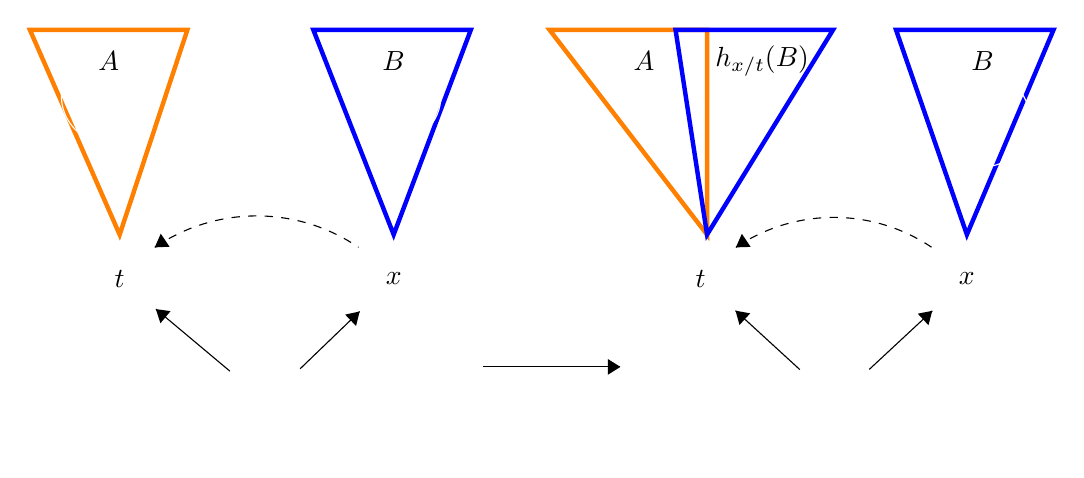
\begin{tikzpicture}[scale=0.2]
\tikzstyle{every node}+=[inner sep=0pt]
\draw [white] (20,-48.6) circle (3);
\draw [white] (10.7,-40.8) circle (3);
\draw (10.7,-40.8) node {$t$};
\draw[orange, ultra thick] (10.7,-38) -- (5,-25) -- (15,-25) -- cycle;
\draw [white] (28.1,-40.8) circle (3);
\draw (28.1,-40.8) node {$x$};
\draw[blue, ultra thick] (28.1,-38) -- (23,-25) -- (33,-25) -- cycle;
\draw [white] (10,-29.2) circle (3);
\draw (10,-27) node {$A$};
\draw [white] (28.1,-29.2) circle (3);
\draw (28.1,-27) node {$B$};
\draw [white] (56.1,-48.6) circle (3);
\draw [white] (47.6,-40.8) circle (3);
\draw (47.6,-40.8) node {$t$};
\draw[orange, ultra thick] (48,-38) -- (38,-25) -- (48,-25) -- cycle;
\draw[blue, ultra thick] (48,-38) -- (46,-25) -- (56,-25) -- cycle;
\draw [white] (64.5,-40.8) circle (3);
\draw (64.5,-40.8) node {$x$};
\draw[blue, ultra thick] (64.5,-38) -- (60,-25) -- (70,-25) -- cycle;
\draw (44,-27) node {$A$};
\draw (51.5,-27) node {$h_{x/t}(B)$};
\draw [white] (65.5,-30.7) circle (3);
\draw (65.5,-27) node {$B$};
\draw [white] (30.8,-46.4) circle (3);
\draw [white] (45.5,-46.4) circle (3);
\draw [black] (17.7,-46.67) -- (13,-42.73);
\fill [black] (13,-42.73) -- (13.29,-43.63) -- (13.93,-42.86);
\draw [black] (22.16,-46.52) -- (25.94,-42.88);
\fill [black] (25.94,-42.88) -- (25.02,-43.08) -- (25.71,-43.8);
\draw [black,dashed] (12.931,-38.807) arc (124.28182:55.71818:11.484);
\fill [black] (12.93,-38.81) -- (13.87,-38.77) -- (13.31,-37.94);
\draw [black] (53.89,-46.57) -- (49.81,-42.83);
\fill [black] (49.81,-42.83) -- (50.06,-43.74) -- (50.74,-43);
\draw [black] (58.3,-46.56) -- (62.3,-42.84);
\fill [black] (62.3,-42.84) -- (61.38,-43.02) -- (62.06,-43.75);
\draw [black,dashed] (49.831,-38.809) arc (124.01582:55.98418:11.116);
\fill [black] (49.83,-38.81) -- (50.77,-38.78) -- (50.21,-37.95);
\draw [black] (33.8,-46.4) -- (42.5,-46.4);
\fill [black] (42.5,-46.4) -- (41.7,-45.9) -- (41.7,-46.9);
\end{tikzpicture}
\end{center}
To prove the result, we will look all the triggers dealing with the variables in $\su(x)$ and apply them on the variables in $\su(t)$ if the triggers have not already been applied.

\begin{proof}
Let $tr_1 = (\alpha_1,\sigma_1),\ldots, tr_n =(\alpha_n,\sigma_n)$ be all the oblivious triggers in $\{trig_1,\ldots,trig_m\}$ such that
\begin{itemize}
\item the range of each $\sigma_i$ contains only variables in $\su(x)$.
\item if $tr_i = trig_r$ and $tr_j =trig_l$, then $i <j$ implies $r<l$ (that is, $tr_1,\ldots,tr_n$ are oredered by application time).
\end{itemize} 
We note $h_{x/t}(tr_i)=(\alpha_i,h_{x/t} \circ \sigma_i)$ and $$B_i' = {h_{x/t} \circ \sigma_1^s}(Head(\alpha_1)) \cup \ldots \cup {h_{x/t} \circ \sigma^s_i}(Head(\alpha_{i}))$$

We show by induction on $i \in \{0,\ldots, n\},H(i)$: There exists oblivious triggers $tr_1',\ldots,tr_r' \in \{h_{x/t} \circ \sigma_1,\ldots, h_{x/t} \circ \sigma_n\}$\todo{Why don't we constructively define this sequence?}\ such that, if we pose $F_{m+1} = \Appl(F_m,tr_1'),\ldots,F_{m+r} = \Appl(F_{m+r-1},tr_r')$, the sequence $D_i = D,tr_1',F_{m+1},\ldots, tr_r',F_{m+r}$ is an oblivious derivation and $B_i' \subseteq F_{m+r}$. 

For i = 0, $D_0 = D$ is an oblivious derivation and $B_0 = \emptyset$, so $H(0)$ is true.

Suppose that $H(i-1)$ is true for $i \in \{1,\ldots,n\}$: $D_{i-1} = D,tr_1',F_{m+1},\ldots, tr_r',F_{m+r}$ is an oblivious derivation and $B_{i-1}' \subseteq F_{m+r}$.\todo{I would merge the last three paragraphs into one.}

Depending on the form of the rule $\alpha_i$, there exists four different cases:
	\begin{itemize}
	\item If $\alpha_i$ is of the form $A(u) \rightarrow \exists v.R(u,v) \wedge B(v)$. We have $A(\sigma_i(u)) \in F_m$.
		\begin{itemize}
		\item If $\sigma_i(u) = x$, then $A(x) \in F_m$. As $t$ is a strong sibling of $x$ in $F_m$, $A(t) \in F_m$. So $A(h_{x/t}(\sigma_i(u))) \in F_{m+r}$ since $h_{x/t}(\sigma_i(u)) = t$.  
		\item If $x \prec^+ \sigma_i(u)$, then the fact $A(\sigma_i(u)))$ has been introduced by an oblivious trigger in $\{tr_1,\ldots,tr_{i-1}\}$. So, by induction hypothesis, $A(h_{x/t}(\sigma_i(u))) \in F_{m+r}$.
		\end{itemize}
Therefore $h_{x/t}(tr_{i})$ is an oblivious trigger for $F_{m+r}$.\todo{Don't you have to check if the trigger has been applied? Also, don't we need to check its applicability to some element that comes before $F_{m+r}$ in the sequence?}

	\item If $\alpha_i$ is of the form $A_1(u) \wedge A_2(u) \rightarrow B(u)$. We have $A_1(\sigma_i(u)),A_2(\sigma_i(u)) \in F_m$.
		\begin{itemize}
		\item If $\sigma_i(u) = x$, then $A_1(x),A_2(x) \in F_m$. As $t$ is a strong sibling of $x$ in $F_m$, we have $A_1(t),A_2(t) \in F_m$. So $A_1(h_{x/t}(\sigma_i(u))),A_2(h_{x/t}(\sigma_i(u))) \in F_{m+r}$ since $h_{x/t}(\sigma_i(u)) = t$.  
		\item If $x \prec^+ \sigma_i(u)$, then the fact $A_1(\sigma_i(u))),A_2(\sigma_i(u)))$ has been introduced by an oblivious trigger in $\{tr_1,\ldots,tr_{i-1}\}$\todo{This part may need a bit more arguing.}. So, by induction hypothesis, $A_1(h_{x/t}(\sigma_i(u))),A_2(h_{x/t}(\sigma_i(u))) \in F_{m+r}$.
		\end{itemize}
Therefore $h_{x/t}(tr_{i})$ is an oblivious trigger for $F_{m+r}$.  

\item If $\alpha_i$ is of the form $A(u) \wedge R(u,v) \rightarrow B(v)$.
	\begin{itemize}
		\item If $\sigma_i(u) = x$, then $A(x) \in F_m$. As $t$ is a strong sibling of $x$ in $F_m$, $A(t)\in F_m$. Thus $A(h_{x/t}(\sigma_i(u))) \in F_{m+r}$.
		\item If $x \prec^+ \sigma_i(u)$, then the fact $A(\sigma_i(u))$ has been introduced by an oblivious trigger in $\{tr_1,\ldots,tr_{i-1}\}$. So, by induction hypothesis, $A(h_{x/t}(\sigma_i(u))) \in F_{m+r}$. 
		\end{itemize}
The fact $R(\sigma_i(u),\sigma_i(v))$ has been introduced by an oblivious trigger in $\{tr_1,\ldots,tr_{i-1}\}$.So by induction hypothesis, $R(h_{x/t}(\sigma_i(u)),h_{x/t}(\sigma_i(v))) \in F_{m+r}$. 

Therefore, the facts $A(\sigma_i(x))$ and $R(\sigma_i(u),\sigma_i(v))$ are in $ F_{m+r}$. Thus $h_{x/t}(tr_{i})$ is an oblivious trigger for $F_{m+r}$.
\item If $\alpha_i$ is of the form $R(u,v) \wedge B(v) \rightarrow A(u)$.

The facts $R(\sigma_i(u),\sigma_i(v)),B(\sigma_i(v))$ has been introduced by an oblivious trigger in $\{tr_1,\ldots,tr_{i-1}\}$. So, by induction hypothesis, the facts $R(h_{x/t}(\sigma_i(u)),h_{x/t}(\sigma_i(v)))$ and $B(h_{x/t}(\sigma_i(v)))$ are in $ F_{m+r}$. Therefore $h_{x/t}(tr_{i})$ is an oblivious trigger for $F_{m+r}$.
	\end{itemize} \todo{I have to add a fifth case for the rule 5}
If $\Appl(F_{m+r},h_{x/t}(tr_{i})) = F_{m+r}$ then $h_{x/t} \circ \sigma_i^s(Head(\alpha_i)) \subseteq F_{m+r}$ so $B_i' = B_{i-1} \cup h_{x/t} \circ \sigma_i^s(Head(\alpha_i)) 	\subseteq F_{m+r}$. Therefore $D_i = D_{i-1}$ is suitable, $H(i)$ is true.

Otherwise, the oblivious trigger $h_{x/t}(tr_{i})$ has not been applied on $F_{m+r}$ we then pose $tr_{r+1}' = h_{x/t}(tr_{i})$, $F_{m+r+1} = \Appl(F_{m+r},tr_{r+1}')$, and $D_i = D_{i-1}, tr_{r+1}',F_{m+r+1}$. As $h_{x/t}(tr_{i})$ is an oblivious trigger for $F_{m+r}$, $D_i$ is an oblivious derivation. By definition of an application, we have $h_{x/t} \circ \sigma_i^s(Head(\alpha_i)) \subseteq F_{m+r+1}$ and so $B_i' = B_{i-1} \cup h_{x/t} \circ \sigma_i^s(Head(\alpha_i)) 	\subseteq F_{m+r}$. Therefore, $H(i)$ is true.


We have proved the heredity. So, $D_n$ is the oblivious derivation that we was looking for. We have $F_{m+n} = F_m \cup h_{x/t}(\Tree_{F_m}(x))$.

\end{proof}


\begin{proposition}
Let $D = F_0,trig_1,F_1,\ldots, trig_m,F_m$ be an oblivious chase derivation of the knowledge base $O$. Assume that $x$ is mergeable on $t$ in $F_m$. The atomic merging of $x$ on $t$ in $F_m$ is a retract of $\Fut(F_m,t,x)$ .
\end{proposition}

\begin{proof}
The atomic merging of $x$ on $t$ in $F_m$ is $h_{x/t}(F_m)$. 

By the Proposition \ref{step1}, $\Fut(F_m,t,x)= F_m \cup h_{x/t}(\Tree_{F_m}(x))$. So, $h_{x/t}(F_m) \subseteq \Fut(F_m,t,x) $ since $\Fut(F_m,t,x) = \Tree_{F_m}(x) \cup h_{x/t}(F_m)$.

As $h_{x/t}(\Fut(F_m,t,x)) = h_{x/t}(F_m)$, we have that $h_{x/t}(F_m) \models \Fut(F_m,t,x)$.\todo{Merge the last three sentences into a single paragraph.}
\end{proof}

The last two propositions shows the following theorem:\todo{The following theorem is a corollary of Propositions 3.5 and 3.6:}\todo{We cannot say that ``a proposition shows''.}

\begin{theorem} \label{universality atomic merge}
The atomic merge is an operation that preserves the universality.\todo{I would make a more precise statement. For instance, I would specify that, when applied to a factbase in an merge chase sequence, the atomic merge operation preserves universality.}
\end{theorem}

The following definition describes the operation that will replace the computation of the core in the core chase. We will show that for a chase derivation $D =F_0,...,F_k$ of $O$, if we apply our operation on $F_k$, then it computes the core of a factbase that could have been produced by continuing the derivation $D$.

\begin{definition}
For a factbase $F$ that occurs in a chase derivation\todo{The notion of a chase derivation has not been introduced yet.}\ of the knowledge base $O$, a \emph{merge} sequence of $F$ is a sequence $F_0,\ldots,F_n$ of factbases such that:
\begin{itemize}
\item $F_0 = F$.
\item For $i \in \{1,\ldots,n\}$, the factbase $F_i$ is the atomic merging of a variable $x$ on a term $t$ in $F_{i-1}$.
\item The factbase $F_n$ does not contain a mergeable variables.
\end{itemize}
Then, $\Merge(F) = F_n$. 
\end{definition}

\begin{example} 
The figure below is an example of merging where we merge the factbase of the left. The variable $f_\alpha^z(a)$ is mergeable on $b$ so we do an atomic merging of $f_\alpha^z(a)$ on $b$ that gives us the factbase of the middle. Now, $f_\beta^z(b)$ is mergeable on $c$ so we do an atomic merging of $f_\beta^z(b)$ on $c$ that gives us the factbase of the right.

\begin{center}
\begin{tikzpicture}[scale=0.2]
\tikzstyle{every node}+=[inner sep=0pt]
\draw [white] (8.2,-36.8) circle (3);
\draw (8.2,-36.8) node {$a:A$};
\draw [white] (4,-24.6) circle (3);
\draw (4,-24.6) node {$b:\mbox{ }C,D$};
\draw [white] (12.2,-24.6) circle (3);
\draw (12.2,-24.6) node {$f_\alpha^z(a):\mbox{ }C$};
\draw [white] (12.2,-11.2) circle (3);
\draw (12.2,-11.2) node {$f_\beta^z(f_\alpha^z(a)):\mbox{ }E$};
\draw [white] (4,-11.2) circle (3);
\draw (4,-11.2) node {$c:\mbox{ }E$};
\draw [white] (15.5,-24.5) circle (3);
\draw [white] (31.1,-24.5) circle (3);
\draw [white] (33.4,-37.6) circle (3);
\draw (33.4,-37.6) node {$a:\mbox{ }A$};
\draw [white] (33.4,-23.8) circle (3);
\draw (33.4,-23.8) node {$b:\mbox{ }C,D$};
\draw [white] (29.3,-11.2) circle (3);
\draw (29.3,-11.2) node {$c:\mbox{ }E$};
\draw [white] (38.1,-11.2) circle (3);
\draw (38.1,-11.2) node {$f_\beta^z(b):\mbox{ }E$};
\draw [white] (35.8,-24.5) circle (3);
\draw [white] (50.5,-24.5) circle (3);
\draw [white] (54.6,-37.6) circle (3);
\draw (54.6,-37.6) node {$a:\mbox{ }A$};
\draw [white] (54.6,-24.5) circle (3);
\draw (54.6,-24.5) node {$b:\mbox{ }C,D$};
\draw [white] (54.6,-11.2) circle (3);
\draw (54.6,-11.2) node {$c:E$};
\draw [black] (7.22,-33.96) -- (4.98,-27.44);
\fill [black] (4.98,-27.44) -- (4.76,-28.36) -- (5.71,-28.03);
\draw (6.86,-29.97) node [right] {$S$};
\draw [black] (4,-21.6) -- (4,-14.2);
\fill [black] (4,-14.2) -- (3.5,-15) -- (4.5,-15);
\draw (4.5,-17.9) node [right] {$R$};
\draw [black] (9.13,-33.95) -- (11.27,-27.45);
\fill [black] (11.27,-27.45) -- (10.54,-28.06) -- (11.49,-28.37);
\draw (10.97,-31.39) node [right] {$S$};
\draw [black] (12.2,-21.6) -- (12.2,-14.2);
\fill [black] (12.2,-14.2) -- (11.7,-15) -- (12.7,-15);
\draw (12.7,-17.9) node [right] {$R$};
\draw [red] (18.5,-24.5) -- (28.1,-24.5);
\fill [red] (28.1,-24.5) -- (27.3,-24) -- (27.3,-25);
\draw [black] (33.4,-34.6) -- (33.4,-26.8);
\fill [black] (33.4,-26.8) -- (32.9,-27.6) -- (33.9,-27.6);
\draw (33.9,-30.7) node [right] {$S$};
\draw [black] (32.47,-20.95) -- (30.23,-14.05);
\fill [black] (30.23,-14.05) -- (30,-14.97) -- (30.95,-14.66);
\draw (32.12,-16.82) node [right] {$R$};
\draw [black] (34.45,-20.99) -- (37.05,-14.01);
\fill [black] (37.05,-14.01) -- (36.3,-14.59) -- (37.24,-14.94);
\draw (36.51,-18.31) node [right] {$R$};
\draw [red] (38.8,-24.5) -- (47.5,-24.5);
\fill [red] (47.5,-24.5) -- (46.7,-24) -- (46.7,-25);
\draw [black] (54.6,-34.6) -- (54.6,-27.5);
\fill [black] (54.6,-27.5) -- (54.1,-28.3) -- (55.1,-28.3);
\draw (55.1,-31.05) node [right] {$S$};
\draw [black] (54.6,-21.5) -- (54.6,-14.2);
\fill [black] (54.6,-14.2) -- (54.1,-15) -- (55.1,-15);
\draw (55.1,-17.85) node [right] {$R$};
\end{tikzpicture}
\end{center}

We can notice that the order of variables we choose is really important because an atomic merging can create mergeable variables. In this example, if we treat $f_\beta^z(f_\alpha^z(a))$ before $f_\alpha^z(a)$, then at the moment where we treat $f_\beta^z(f_\alpha^z(a))$, it does not have any term $t$ yet such that $f_\beta^z(f_\alpha^z(a))$ is mergeable on $t$ so at the end, we get the factbase of the middle and we will not have merged every possible mergeable variable.\todo{Nice example!}
\end{example}

The merge operation uses only atomic merge\todo{Minor problem here: the results re. the universality of atomic merging can only be applied to fact sets that occur during the computation of the oblivious chase.}, so by Theorem \ref{universality atomic merge}:

\begin{theorem} \label{universality merge}
The merge is an operation that preserves the universality.
\end{theorem}

We will now consider a new chase:

\begin{definition}[derivation]
A \emph{merge derivation} for a knowledge base $O = (R,F)$ is a (possibly infinite) sequence $D = F_0, F_1, F_2, \ldots$ where $F_0 = F$, and for $i >0$, either $F_{i}= \Appl(F_{i-1},t_i)$ is obtained by an application with $t_i$ an oblivious trigger, or $F_i = \Merge(F_{i-1})$ is obtained by the merging of $F_{i-1}$ . 
\end{definition} 

\begin{definition}[derivation]
A merge derivation $D = F_0, F_1, F_2, \ldots$ for a knowledge base $O = (R,F)$ is \emph{fair} if: 
\begin{itemize}
\item For every $i$, for every oblivious trigger $t$ applicable on $F_i$, there exists $k > i$ such that $\Appl(F_{k},t) = F_k$.\todo{Problem here: the merging operation will remore things! Messes up with ths notion of fairness.}
\item For every $i$, there exists $k \geq i$ such that $F_k$ is a core.
\end{itemize}
\end{definition} 

\begin{definition}
A \emph{merge chase} for a knowledge base $O= (R,F)$ is a fair atomic merge derivation $D=F_0,F_1,F_2,\ldots$
\end{definition}

\begin{definition}
The merge chase $D=F_0,F_1,F_2,\ldots$ \emph{terminates} on $O$ if it is a finite derivation. We pose: \todo{}
\end{definition}




It is really important that the merging does all the possible atomic merging that it can do. Otherwise, the merge chase may not terminates on some knowledge base whereas there exists a finite universal model (like in the next example) and we want that the merge chase terminates on all knowledge base that admits a finite universal model.\todo{Bit of a long sentence.}

\begin{example} \label{necessity of atomic merge}
We consider in the example that $F= \{R(a,b),R(b,a),A(a),A(b)\}$ and $R = \{\alpha, \beta\}$ where $\alpha = A(x) \rightarrow \exists y.R(x,y) \wedge A(y)$ and $\beta=B(x) \rightarrow A(x)$. We consider the atomic merge chase derivation $F_0 =F,F_1,F_2,...$ We applied to $F_0$ the oblivious trigger $t_1 = (\alpha, \{x \mapsto a\})$, we then applied to $F_1$, the oblivious trigger $t_2 = (\alpha, \{x \mapsto f_\alpha^y(a)\})$ giving rise to the first factbase of the figure below. We then apply the oblivious trigger $t_3 = (\beta, \{x \mapsto b\})$ to obtain the factbase $F_3$. At this moment, $f_\alpha^y(a)$ is mergeable on $b$ so we do an atomic merging of $f_\alpha^y(a)$ on $b$ to get $F_4$ that is the second factbase of the figure. $F_5$ is obtained by the application of the oblivious trigger $t_4 = (\alpha, \{x \mapsto f_\alpha^y(b)\})$ and is the third factbase of the figure. At this moment, $f_\alpha^y(b)$ is mergeable on $a$ so we do an atomic merging of $f_\alpha^y(b)$ on $a$ to get $F_6$ that is the last factbase of the figure. We can repeat this infinitely. But $O$ admits a finite universal model: $U = F \cup \{B(b)\}$. So the version of the chase where we consider partial merging is not what we want.

\todo{changer l'example -> why?}
\begin{center}
\begin{tikzpicture}[scale=0.2]
\tikzstyle{every node}+=[inner sep=0pt]
\draw [white] (8.5,-24.6) circle (3);
\draw (8.5,-24.6) node {$a:\mbox{ }A$};
\draw [white] (8.5,-33.9) circle (3);
\draw (8.5,-33.9) node {$b:\mbox{ }B$};
\draw [white] (8.5,-14.8) circle (3);
\draw (8.5,-14.8) node {$f_\alpha^y(a):\mbox{ }A$};
\draw [white] (8.5,-5.4) circle (3);
\draw (8.5,-5.4) node {$f_\alpha^y(f_\alpha^y(a)):\mbox{ }A$};
\draw [white] (24.7,-33.9) circle (3);
\draw (24.7,-33.9) node {$b:\mbox{ }A,B$};
\draw [white] (24.7,-24) circle (3);
\draw (24.7,-24) node {$a:A$};
\draw [white] (24.7,-44.2) circle (3);
\draw (24.7,-44.2) node {$f_\alpha^y(b):\mbox{ }A$};
\draw [white] (40,-44.2) circle (3);
\draw (40,-44.2) node {$f_\alpha^y(b):\mbox{ }A$};
\draw [white] (40,-33.9) circle (3);
\draw (40,-33.9) node {$b:\mbox{ }A,B$};
\draw [white] (40,-24) circle (3);
\draw (40,-24) node {$a:\mbox{ }A$};
\draw [white] (40,-54.1) circle (3);
\draw (40,-54.1) node {$f_\alpha^y(f_\alpha^y(b)):\mbox{ }A$};
\draw [white] (55.7,-24.6) circle (3);
\draw (55.7,-24.6) node {$a:\mbox{ }A$};
\draw [white] (55.7,-34.5) circle (3);
\draw (55.7,-34.5) node {$b:\mbox{ }A,B$};
\draw [white] (55.7,-14.8) circle (3);
\draw (55.7,-14.8) node {$f_\alpha^y(a):\mbox{ }A$};
\draw [white] (11.9,-28.9) circle (3);
\draw [white] (20.5,-28.9) circle (3);
\draw [white] (28.6,-28.8) circle (3);
\draw [white] (36.9,-28.8) circle (3);
\draw [white] (44,-28.8) circle (3);
\draw [white] (52.7,-28.8) circle (3);
\draw [white] (58.6,-29.9) circle (3);
\draw [white] (67.2,-29.9) circle (3);
\draw (67.2,-29.9) node {$\ldots$};
\draw [black] (11.162,-25.868) arc (46.19008:-46.19008:4.686);
\fill [black] (11.16,-25.87) -- (11.39,-26.78) -- (12.09,-26.06);
\draw (13.1,-29.25) node [right] {$R$};
\draw [black] (5.784,-32.753) arc (-131.32879:-228.67121:4.664);
\fill [black] (5.78,-32.75) -- (5.51,-31.85) -- (4.85,-32.6);
\draw (3.7,-29.25) node [left] {$R$};
\draw [black] (8.5,-21.6) -- (8.5,-17.8);
\fill [black] (8.5,-17.8) -- (8,-18.6) -- (9,-18.6);
\draw (9,-19.7) node [right] {$R$};
\draw [black] (8.5,-11.8) -- (8.5,-8.4);
\fill [black] (8.5,-8.4) -- (8,-9.2) -- (9,-9.2);
\draw (9,-10.1) node [right] {$R$};
\draw [black] (27.299,-25.408) arc (44.53872:-44.53872:5.05);
\fill [black] (27.3,-25.41) -- (27.5,-26.33) -- (28.22,-25.63);
\draw (29.25,-28.95) node [right] {$R$};
\draw [black] (22.29,-32.183) arc (-141.88061:-218.11939:5.237);
\fill [black] (22.29,-32.18) -- (22.19,-31.24) -- (21.4,-31.86);
\draw (20.67,-28.95) node [left] {$R$};
\draw [black] (24.7,-36.9) -- (24.7,-41.2);
\fill [black] (24.7,-41.2) -- (25.2,-40.4) -- (24.2,-40.4);
\draw (24.2,-39.05) node [left] {$R$};
\draw [black] (42.676,-25.254) arc (47.68401:-47.68401:4.998);
\fill [black] (42.68,-25.25) -- (42.93,-26.16) -- (43.6,-25.42);
\draw (44.81,-28.95) node [right] {$R$};
\draw [black] (40,-47.2) -- (40,-51.1);
\fill [black] (40,-51.1) -- (40.5,-50.3) -- (39.5,-50.3);
\draw (39.5,-49.15) node [left] {$R$};
\draw [black] (40,-36.9) -- (40,-41.2);
\fill [black] (40,-41.2) -- (40.5,-40.4) -- (39.5,-40.4);
\draw (39.5,-39.05) node [left] {$R$};
\draw [black] (37.553,-32.236) arc (-140.75683:-219.24317:5.195);
\fill [black] (37.55,-32.24) -- (37.43,-31.3) -- (36.66,-31.93);
\draw (35.88,-28.95) node [left] {$R$};
\draw [black] (53.409,-32.624) arc (-145.24527:-214.75473:5.392);
\fill [black] (53.41,-32.62) -- (53.36,-31.68) -- (52.54,-32.25);
\draw (51.95,-29.55) node [left] {$R$};
\draw [black] (58.055,-26.393) arc (36.51301:-36.51301:5.305);
\fill [black] (58.06,-26.39) -- (58.13,-27.33) -- (58.93,-26.74);
\draw (59.6,-29.55) node [right] {$R$};
\draw [black] (55.7,-21.6) -- (55.7,-17.8);
\fill [black] (55.7,-17.8) -- (55.2,-18.6) -- (56.2,-18.6);
\draw (56.2,-19.7) node [right] {$R$};
\draw [red] (14.9,-28.9) -- (17.5,-28.9);
\fill [red] (17.5,-28.9) -- (16.7,-28.4) -- (16.7,-29.4);
\draw [red] (31.6,-28.8) -- (33.9,-28.8);
\fill [red] (33.9,-28.8) -- (33.1,-28.3) -- (33.1,-29.3);
\draw [red] (47,-28.8) -- (49.7,-28.8);
\fill [red] (49.7,-28.8) -- (48.9,-28.3) -- (48.9,-29.3);
\draw [red] (61.6,-29.9) -- (64.2,-29.9);
\fill [red] (64.2,-29.9) -- (63.4,-29.4) -- (63.4,-30.4);
\end{tikzpicture}
\end{center}
\end{example}



We want now prove that a merging computes a core:

\begin{proposition} \label{core}
For a factbase $G$ obtained by applying some Horn-$\mathcal{ALCH}$ axioms on $O$, $\Merge(G)$ is a core.
\end{proposition}

\begin{proof}
%\item The $\mathcal{ALCH}$-pruning algorithm only take off facts of the factbase. Consequently, $\textit{prune}(G) \subseteq G$.
%\item We consider the homorphism $h:G \to \textit{prune}(G)$ created during the $\mathcal{ALCH}$-pruning algorithm. For $x \in \Vars(G)$, suppose that $h(x) \neq x$. According to the $\mathcal{ALCH}$-pruning algorithm, $x$ has been erased \todo{à préciser}. So $x \notin \Vars(\textit{prune}(G))$. So ${h}_{|\textit{Prune}(G)}=id_{|\textit{Prune}(G)}$. We have shown that $h$ is a retract so $\textit{prune}(G)$ is a retract of $G$.
Suppose for a contradiction that $\Merge(G)$ is not a core. There exists $G' \subsetneq \Merge(G)$ such that $G'$ is a retract of $\Merge(G)$. By Proposition \cite{retract}\todo{Use "href" instead of "cite".}, there exists then a retractation $h$ from $\Merge(G)$ to $G'$. We have $var(\Merge(G))\setminus var(G') \neq \emptyset$. Let $x$ be a $\prec$-minimal variable of this set. The term $x$ is a variable, so has been introduced by the chase due to the axiom 3\todo{Rule of the form (3).}. So there exists a term $t$ such that $t \prec x$. 
\begin{itemize}
\item We have $\Preds^2_{\Merge(G)}(t,x) \neq \emptyset$. By $\prec$-minimality of $x$, $t \in \Vars(G')$. So, as $h$ is a retractation: $h(t) = t$, so for $R \in \Preds^2_{\Merge(G)}(t,x)$, $h(R(t,x)) = R(t,h(x)) \in \Merge(G)$ and so $R \in \Preds^2_{\Merge(G)}(t,h(x))$. Thus $\Preds^2_{\Merge(G)}(t,x) \subseteq \Preds^2_{\Merge(G)}(t,h(x))$ and $t \prec h(x)$.
\item $x \notin G'$ and $h(x) \in G'$ so $h(x) \neq x$. 
\item Let $A \in \Preds^1_{\Merge(G)}(x)$. $h(A(x)) \in \Merge(G)$ so $A(h(x)) \in \Merge(G)$ so $\Preds^1_{\Merge(G)}(x) \subseteq \Preds^1_{\Merge(G)}(h(x))$. 
\end{itemize}
Consequently, $x$ is mergeable on $h(x)$ in $\Merge(G)$: contradiction\todo{which results on a contradiction}. So\todo{He} $\Merge(G)$ is a core.
\end{proof}	

$\Merge(G)$ is a core but not necessarily the core of $G$.


%\begin{definition}
%$tr = (\alpha,\sigma, \hat \sigma)$ is a \emph{stupid trigger} if $(\alpha,\sigma)$ is an oblivious trigger, and if $\hat \sigma$ extends $\sigma$ and is defined on $\Vars(\textit{Head}(\alpha))$. The factbase $\Appl(F,tr)=F \cup \hat \sigma(\textit{Head}(\alpha))$ is called an \emph{application} on the factbase $F$ through the stupid trigger $tr = (\alpha,\sigma, \hat \sigma)$. A \emph{stupid derivation} from a knowledge base $O= (F,R)$ is a (possibly infinite) sequence $D=F_0,tr_1,F_1,tr_2,F_2,\ldots$ where $(F_i)_{i \in \N}$ are factbases, $tr_i$ are stupid triggers, $F_0 = F$, and for $i >0$, $F_{i}= \Appl(F_{i-1},tr_i)$ is obtained by an application. The stupid derivation $D=F_0,t_1,F_1,t_2,F_2,\ldots$ is \emph{fair} if for every $i$ and every stupid trigger $tr = (\alpha,\sigma, \hat \sigma)$ applicable on $F_i$, there exists $k \geq i$ such that there exists a stupid trigger $tr' = (\alpha,\sigma, \hat \sigma')$ that verified $\Appl(F_{k},tr') = F_k$. A \emph{stupid chase} for a knowledge base $O= (F,R)$ is a fair stupid derivation $D=F_0,tr_1,F_1,tr_2,F_2,\ldots$ $F_0 \subseteq F_1 \subseteq F_2 \subseteq \ldots$ so we can pose \emph{$\textit{Stp(O)}$} = $\cup_{i \in \N}F_i$.
%We say that the stupid chase \emph{terminates} if $\textit{Stp(O)}$ is finite.
%\end{definition}




\begin{proposition}
The merge chase computes a finite universal model of $O$ when it terminates.
\end{proposition}

\begin{proof}
Let $D = F_0,\ldots,F_n$ be a merge chase for $O =(R,G)$. 
\begin{itemize}
\item The merge chase never take off ground facts and $G =F_0$ so $G \subseteq F_n$. We have then $F_n \models G$. Assume for a contradiction that $F_n \nvDash R$. There exists then a rule $\alpha$ in $R$ not satisfied by $F_n$: $F_n \vDash \textit{Body}(\alpha)$ and $F_n \nvDash \textit{Head}(\alpha)$. It means that there exists a substitution $\sigma$ from $\textit{Body}(\alpha)$ to $F_n$. Therefore, $t=(\alpha,\sigma)$ is an oblivious trigger for $F_n$. As the derivation $D$ is fair, $\Appl(F_n,t) = F_n$. Thus $\sigma^s(\textit{Head}(\alpha)) \subseteq F_n$ and so $F_n \models \alpha$: contradiction. We have then $F_n \models R$ so $F_n$ is a model of $O$.\todo{What if the atoms of the head are removed bc of a merge operation? This needs to be briefly discussed.}
\item According to Proposition \ref{universality application} and \ref{universality merge}, each operation of the merge chase conserves the universality so we can show by induction that $F_n$ is a universal model of $O$.
\item We applied a finite number of operations and each operation either add a finite number of facts or remove facts so $F_n$ is finite.\todo{This sentence can be ignored.}
\end{itemize}
\end{proof}

\begin{proposition}
If there exists a finite universal model for $O$, the merge chase terminates.
\end{proposition}

\begin{proof}

\end{proof}


\begin{theorem}
The merge chase computes an universal model if and only if there exists an universal model.
\end{theorem}

We will now describe a deterministic algorithm to merge a factbase:

\begin{definition}[Merging]
Let $F$ be a factbase that occurs in a chase derivation of the knowledge base $O$.

\begin{algorithm}[H]
\SetAlgoLined


    Let $\textbf{\Vars}(F) = \{x_1,\ldots, x_n\}$ be such that $(x_i \prec^+ x_j) \Rightarrow i < j$ \;
    \For{$i =1 \text{ to } n$}{
    	\If{$x_i$ is still a variable in $F$}{
			\For{all term $t$ such that $x_i$ is mergeable on $t$}{
				$F \leftarrow$ the atomic merging of $x_i$ on $t$ in $F$.
			}
		}
	}
return $F$
\caption{Merge($F$):}


\end{algorithm}
At line 1, we can sort terms like that because, by proposition \ref{partial_order}, $\prec^+$ is a strict partial order over the set of variables of $F$.
\end{definition}

The Example \ref{necessity of atomic merge} shows the importance of doing a total merging. We have to prove that our merging algorithm does a total merging:

\begin{proposition}\label{no_more_siblings}
Let $G$ be a factbase that occurs in a chase derivation of the knowledge base $O$. There does not exists a term $t$ and a variable $x$ such that $x$ is mergeable on $t$ in $\Merge(G)$.
\end{proposition}

\begin{proof} \todo{I have to modify some stuff for rule 5}
Suppose for a contradiction that there exists a term $t$ and a variable $x$ such that $x$ is mergeable on $t$ in $\Merge(G)$, that is, there exists a term $t'$ and a binary predicate $R$ such that $R(t',x),R(t',t) \in \Merge(G)$. This case can happen only if $x$ became mergeable  after that $x$ has been traited by the merging algorithm. Thus, during the merging, there has been an atomic merging on $t'$. Let $y$ be the variable merged on $t'$ such that $y \prec x$. We note $G^1$ the factbase just before the atomic merging of $y$ on $t'$ and we note $G^2$ the factbase just after the atomic merging. There exists a term $t_0$ and a binary predicate $S$ such that $S(t_0,t'),S(t_0,y) \in G^1$. $G^1$ is the left figure and $G^2$ is the right figure (we do not represent all the graphs):

\begin{center}
\begin{tikzpicture}[scale=0.2]
\tikzstyle{every node}+=[inner sep=0pt]
%\filldraw[color=red!60, fill=red!5, very thick](17,-38) circle (6);
%\filldraw[color=red!60, fill=red!5, very thick](60,-39) circle (6);
%\filldraw[color=red!60, fill=red!5, very thick](10,-11) circle (4);
%\filldraw[color=red!60, fill=red!5, very thick](25,-11) circle (4);
%\filldraw[color=red!60, fill=red!5, very thick](65,-11) circle (4);
%\filldraw[color=red!60, fill=red!5, very thick](54,-11) circle (4);
\draw [white] (17.1,-35.9) circle (3);
\draw (17.1,-35.9) node {$t_0$};
\draw [white] (10.1,-24.1) circle (3);
\draw (10.1,-24.1) node {$t'$};
\draw [white] (24.1,-24.1) circle (3);
\draw (24.1,-24.1) node {$y$};
\draw [white] (24.1,-12.4) circle (3);
\draw (24.1,-12.4) node {$x$};
\draw [white] (10.1,-12.4) circle (3);
\draw (10.1,-12.4) node {$t$};
\draw [white] (30.7,-24.6) circle (3);
\draw [white] (50.4,-24.6) circle (3);
\draw [white] (59.7,-36.8) circle (3);
\draw (59.7,-36.8) node {$t_0$};
\draw [white] (59.7,-25.3) circle (3);
\draw (59.7,-25.3) node {$t'$};
\draw [white] (53.4,-13.2) circle (3);
\draw (53.4,-13.2) node {$t$};
\draw [white] (65.4,-13.2) circle (3);
\draw (65.4,-13.2) node {$x$};
\draw [black] (15.57,-33.32) -- (11.63,-26.68);
\fill [black] (11.63,-26.68) -- (11.61,-27.62) -- (12.47,-27.11);
\draw (14.25,-28.75) node [right] {$S$};
\draw [black] (10.1,-21.1) -- (10.1,-15.4);
\fill [black] (10.1,-15.4) -- (9.6,-16.2) -- (10.6,-16.2);
\draw (10.6,-18.25) node [right] {$R$};
\draw [black] (18.63,-33.32) -- (22.57,-26.68);
\fill [black] (22.57,-26.68) -- (21.73,-27.11) -- (22.59,-27.62);
\draw (21.25,-31.25) node [right] {$S$};
\draw [black] (24.1,-21.1) -- (24.1,-15.4);
\fill [black] (24.1,-15.4) -- (23.6,-16.2) -- (24.6,-16.2);
\draw (24.6,-18.25) node [right] {$R$};
\draw [black] (33.7,-24.6) -- (47.4,-24.6);
\fill [black] (47.4,-24.6) -- (46.6,-24.1) -- (46.6,-25.1);
\draw [black] (59.7,-33.8) -- (59.7,-28.3);
\fill [black] (59.7,-28.3) -- (59.2,-29.1) -- (60.2,-29.1);
\draw (60.2,-31.05) node [right] {$S$};
\draw [black] (58.31,-22.64) -- (54.79,-15.86);
\fill [black] (54.79,-15.86) -- (54.71,-16.8) -- (55.6,-16.34);
\draw (57.24,-18.11) node [right] {$R$};
\draw [black] (60.98,-22.59) -- (64.12,-15.91);
\fill [black] (64.12,-15.91) -- (63.33,-16.42) -- (64.23,-16.85);
\draw (63.26,-20.3) node [right] {$R$};
\end{tikzpicture}
\end{center}

We have $t_0 \prec t' \prec t$ and $t_0 \prec y \prec x$ so $x$ should have been treated by the algorithm after the merging of $t'$ and $y$ so the algorithm will merge $x$ on $t$: contradiction. 
\end{proof}


\subsection{Horn-$\mathcal{ALCHI}$}

\begin{definition}[Horn-$\mathcal{ALCHI}$ axioms]
A \emph{Horn-$\mathcal{ALCHI}$ axiom} is either a Horn-$\mathcal{ALCH}$ axiom or an existential rule of the form:
\begin{align}
R_1(x,y) \wedge R_2(x,y) \rightarrow S(y,x)
\end{align}

\end{definition}



We fix $O=(R,F)$ a knowledge base for this section where $R$ is a Horn-$\mathcal{ALCHI}$ rule set and F is a ground factbase with predicates of arity one or two. We have to modify the merge chase because it doesn't work anymore:

We keep the same relation $\prec$. It is still a strict partial order over the set of variables.



\bibliographystyle{plain}
\bibliography{sample}


\end{document}









tree-like structure 

\begin{definition}[Entailment]
A factbase F \emph{entails} a factbase F' (often noted F $\models F'$) if for all model M de T, M is a model of F'. 
\end{definition}

Let $\prec$ be a strict total order over the set of variables. A variable x occuring in a factbase F is \emph{superfluous} if there exists two variables y and z such that:
\begin{itemize}
\item For all unary predicate P such that $P(x) \in F$, $P(y) \in F$.
\item For all binary predicate R such that $R(z,x) \in F$, $R(z,y) \in F$
\end{itemize}
The \emph{pruning sequence} of a factbase F is the sequence $(F_i)_{i \in \{1,\ldots,n\}}$ of factbases where:
\begin{itemize}
\item $F_1 = F$;
\item for all $i \in \{2,\ldots,n\}$, $F_i$ is the set obtained when we remove every fact of $F_{i-1}$  that contains the smallest superfluous variable (smallest according to $\prec$).
\item $F_n$ does not contain any superfluous variables.
\end{itemize}
We pose \emph{prune(F)} = $F_n$.